\documentclass[]{article}
\usepackage{lmodern}
\usepackage{amssymb,amsmath}
\usepackage{ifxetex,ifluatex}
\usepackage{fixltx2e} % provides \textsubscript
\ifnum 0\ifxetex 1\fi\ifluatex 1\fi=0 % if pdftex
  \usepackage[T1]{fontenc}
  \usepackage[utf8]{inputenc}
\else % if luatex or xelatex
  \ifxetex
    \usepackage{mathspec}
  \else
    \usepackage{fontspec}
  \fi
  \defaultfontfeatures{Ligatures=TeX,Scale=MatchLowercase}
\fi
% use upquote if available, for straight quotes in verbatim environments
\IfFileExists{upquote.sty}{\usepackage{upquote}}{}
% use microtype if available
\IfFileExists{microtype.sty}{%
\usepackage{microtype}
\UseMicrotypeSet[protrusion]{basicmath} % disable protrusion for tt fonts
}{}
\usepackage[margin=1in]{geometry}
\usepackage{hyperref}
\hypersetup{unicode=true,
            pdftitle={Opening up the court (surface) in tennis grand slams},
            pdfborder={0 0 0},
            breaklinks=true}
\urlstyle{same}  % don't use monospace font for urls
\usepackage{graphicx,grffile}
\makeatletter
\def\maxwidth{\ifdim\Gin@nat@width>\linewidth\linewidth\else\Gin@nat@width\fi}
\def\maxheight{\ifdim\Gin@nat@height>\textheight\textheight\else\Gin@nat@height\fi}
\makeatother
% Scale images if necessary, so that they will not overflow the page
% margins by default, and it is still possible to overwrite the defaults
% using explicit options in \includegraphics[width, height, ...]{}
\setkeys{Gin}{width=\maxwidth,height=\maxheight,keepaspectratio}
\IfFileExists{parskip.sty}{%
\usepackage{parskip}
}{% else
\setlength{\parindent}{0pt}
\setlength{\parskip}{6pt plus 2pt minus 1pt}
}
\setlength{\emergencystretch}{3em}  % prevent overfull lines
\providecommand{\tightlist}{%
  \setlength{\itemsep}{0pt}\setlength{\parskip}{0pt}}
\setcounter{secnumdepth}{5}
% Redefines (sub)paragraphs to behave more like sections
\ifx\paragraph\undefined\else
\let\oldparagraph\paragraph
\renewcommand{\paragraph}[1]{\oldparagraph{#1}\mbox{}}
\fi
\ifx\subparagraph\undefined\else
\let\oldsubparagraph\subparagraph
\renewcommand{\subparagraph}[1]{\oldsubparagraph{#1}\mbox{}}
\fi

%%% Use protect on footnotes to avoid problems with footnotes in titles
\let\rmarkdownfootnote\footnote%
\def\footnote{\protect\rmarkdownfootnote}

%%% Change title format to be more compact
\usepackage{titling}

% Create subtitle command for use in maketitle
\newcommand{\subtitle}[1]{
  \posttitle{
    \begin{center}\large#1\end{center}
    }
}

\setlength{\droptitle}{-2em}

  \title{Opening up the court (surface) in tennis grand slams}
    \pretitle{\vspace{\droptitle}\centering\huge}
  \posttitle{\par}
    \author{}
    \preauthor{}\postauthor{}
      \predate{\centering\large\emph}
  \postdate{\par}
    \date{September 15, 2018}

\usepackage{booktabs}
\usepackage{longtable}
\usepackage{array}
\usepackage{multirow}
\usepackage[table]{xcolor}
\usepackage{wrapfig}
\usepackage{float}
\usepackage{colortbl}
\usepackage{pdflscape}
\usepackage{tabu}
\usepackage{threeparttable}
\usepackage{threeparttablex}
\usepackage[normalem]{ulem}
\usepackage{makecell}

\usepackage{hyperref}

\begin{document}
\maketitle
\begin{abstract}
Tennis grand slams consist of the Australian Open, French Open,
Wimbledon, and US Open, which are played on hard (Plexicushion), clay,
grass, and hard (DecoTurf) courts, respectively. The surface type may
substantially impact ball speed, height, and spin as well as player
speed and agility. It is also believed that play style and practice
habits may contribute to different results across surface types. For
example, Rafael Nadal is thought to be the best clay court player of all
time whereas Roger Federer is particularly known for dominance at
Wimbledon. On the women's side, Serena Williams once struggled on clay
courts but has seemingly transformed her style to perform better on clay
courts, but has perhaps suffered on grass as a consequence. In this
analysis, we examine the result of the top 100 players in grand slams
from 2013-2017 across the four different surfaces. We create a
hierarchical model with fixed and random effects to predict the number
of points won in a match. We take into consideration player-specific
effects, nationality (which is thought to have an effect on play style),
sex, ranking, ELO, and game statistics. We assess the fit of our model
using standard statistical techniques (e.g.~MSE, AIC, BIC, residual
diagnostics) in addition to `common knowledge' factors (for instance,
Rafael Nadal should be indicated as a superior clay court player by the
model). We compare the results of top 100 players across grand slams to
examine the effect of court surface. We also provide an in-depth
analysis of Nadal, Federer, and S. Williams.
\end{abstract}

{
\setcounter{tocdepth}{2}
\tableofcontents
}
\hypertarget{sec:iintro}{%
\section{Introduction}\label{sec:iintro}}

Rafael Nadal is known as the ``King of Clay'' in tennis, having won 11
out of his current 17 grand slams titles at the French Open, which is
played on a clay surface (Jurejko 2018). In contrast, his rival Roger
Federer has won his most grand slam titles (8 out of 20) at Wimbledon,
which is played on grass. On the women's side, Serena Williams, winner
of 24 grand slam titles, has been dominant both on hard court (7 titles
at the Australian Open and 6 at US Open) and grass (7 at Wimbledon).
This trend extends to other top players, who seem to have better results
at some grand slams than others. More broadly, it seems that country of
origin has an interaction effect with court type. For example, Spanish
players seem to excel on clay courts and Americans have great success at
Wimbledon despite grass courts not being of wide use in the USA. It also
worth questioning whether the US Open and Australian Open should be
grouped together as hard courts despite having different surface
compositions (Paxinos 2007). In this paper, we analyze the results of
grand slam players from 2013-2017, and we

\begin{enumerate}
\def\labelenumi{\arabic{enumi}.}
\item
  Determine if and how court surface effects players by implementation
  of a series of nested hierarchical models
\item
  Examine how Nadal, Federer, and Williams' play differs by surface
\item
  Assess whether we can group the two hard court surfaces together.
\end{enumerate}

As to issue (1) quantifying the effect of court surface on players,
there has not been much written about with regards to tennis. There are
materials available in the literature for forecasting the outcome of
tennis matches (Klaassen and Magnus 2003; Newton and Keller 2005; McHale
and Morton 2011; Kovalchik 2016){]} or for assessing whether points
within a match are independent and identically distributed (Klaassen and
Magnus 2001). (Knottenbelt, Spanias, and Madurska 2012) do take into
account surface in their model but do not compare the results of one
surface to another. Other sports analyses do take into account surface
type such as grass vs.~turf in soccer and football. Results from these
studies show that surface type does have an effect on the game, either
directly or indirectly {[}Andersson, Ekblom, and Krustrup (2008); Gains
et al. (2010);{]}.

We use models that take into account both individual and group effects
such as in the Gaussian-process player production basketball model or
predicting individual soccer performance (Page, Barney, and McGuire
2013; Egidi and Gabry 2018). Both of those models had success using
hierarchical Bayesian models, which we employ in our own models. More
specifically, we model the players' expected points in a match based on
the player's own characteristics, the court/tournament effects, and the
opponent's ranking.

For issue (2) the player analysis of Nadal, Federer, and Williams, we
examine whether our model passes the ``common sense'' tests like how the
models in (Thomas et al. 2013) show that commonly well known hockey
players also have high status in the model. We also examine whether
these players do have surface apparent effects. Few academic papers have
been written about Nadal, Federer, or Williams. One paper studies
Federer's odds of winning when Nadal suddenly withdrew from Wimbledon
showed that Federer was too heavily favored by bookmakers (Leitner,
Zeileis, and Hornik 2009). One analysis of Williams shows how she has
gotten better with age, even past the point when other greats began to
decline, but the study does not look at surface type (Morris 2015).

Finally, for issue (3), we use clustering methods in order to determine
which court surface types are more similar to one another.

Readers may object that we are looking at differences between grand
slams, which each have their own time period, weather conditions, play
time conditions, and ``home court effects'' instead of differences in
surfaces alone. However, (1) grand slam data is the most readily
available and most complete which makes it the best choice at the moment
for modelling, (2) we adjust for these confounders where we can, and (3)
analyzing the difference in the grand slams is still useful as they are
considered to be the most prestigious events in tennis.

The rest of this paper is organized as follows. In
\protect\hyperlink{sec:data}{Section Data} we describe our grand slam
tennis data. In \protect\hyperlink{sec:eda}{Section Early Data Analysis}
we examine the data at a high level and use clustering whether to
determine how the courts differ from one another. In
\protect\hyperlink{sec:methods}{Section Methods} we describe our
hierarchical models we use to determine difference in court surfaces. In
\protect\hyperlink{sec:results}{Section Results} we describe the results
of our modelling and also examine the play of Nadal, Federer, and
Williams. Finally in \protect\hyperlink{discussion}{Section Discussion},
we discuss future work and extensions or our model.

\hypertarget{sec:data-eda}{%
\section{Data and EDA}\label{sec:data-eda}}

\hypertarget{sec:data}{%
\subsection{Data}\label{sec:data}}

The data consists of 5080 matches split evenly over the four grand slams
and the two leagues: ATP (men's) and WTA (women's). Each match has 80
attributes, many of which are redundant. We focus on the following
attributes for both the winner and loser of the match: games won, points
won, retirement, break points faced, break points saved, aces, country
of origin, and player attributes. Additionally, we take into account the
number of sets in a match, the surface type, and round of the
tournament. A subset of the data is shown in Table \ref{tab:data}.

\rowcolors{2}{gray!6}{white}
\begin{table}

\caption{\label{tab:tab-data}\label{tab:data}Example of the grand slam data.  It includes winner and loser attributes, match attributes, and tournament attributes.  Not all attributes are shown here.}
\centering
\begin{tabular}[t]{llrlrrrr}
\hiderowcolors
\toprule
Winner & Tournament & Year & W. IOC & W. Points & W. Rank & L. Points & L. Rank\\
\midrule
\showrowcolors
Serena Williams & Australian Open & 2013 & USA & 52 & 3 & 18 & 110\\
Serena Williams & Australian Open & 2013 & USA & 70 & 3 & 41 & 112\\
Roger Federer & Australian Open & 2013 & SUI & 95 & 2 & 63 & 46\\
Roger Federer & Australian Open & 2013 & SUI & 111 & 2 & 86 & 40\\
Rafael Nadal & Roland Garros & 2013 & ESP & 140 & 4 & 115 & 59\\
Rafael Nadal & Roland Garros & 2013 & ESP & 113 & 4 & 90 & 35\\
\bottomrule
\end{tabular}
\end{table}
\rowcolors{2}{white}{white}

The data is obtained from Jeff Sackmann's open website via the
\texttt{R} package \texttt{deuce} (Sackmann 2018; Kovalchik 2017). All
steps of our analysis from collection to dissemination are freely
available online.

\hypertarget{sec:eda}{%
\subsection{Early Data Analysis}\label{sec:eda}}

\hypertarget{examining-the-distribution-of-points-earned}{%
\subsubsection{Examining the distribution of points
earned}\label{examining-the-distribution-of-points-earned}}

We first examine the distribution of points earned per match to assess
normality. The distribution of points earned is approximately normal.
This distribution is similar across tournament, with Wimbledon differing
slightly from the other grand slams. As expected, there are more points
earned in the WTA than the ATP due to the differing numbers of games
played. Also unsurprisingly, the winners of the match tended to earn
more points than the losers.

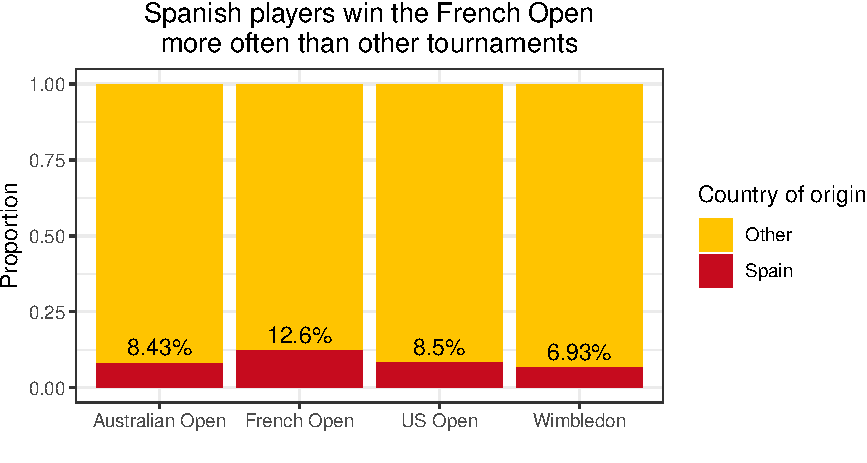
\includegraphics{paper-tennis_files/figure-latex/unnamed-chunk-1-1.pdf}

\hypertarget{home-court-advantage}{%
\subsubsection{Home court advantage}\label{home-court-advantage}}

It is commonly thought that there is a home court advantage in grand
slam games (SOURCE). In our data we find this to be true (i.e.~French
players win the French open more than French players win other slams).
But, we also know that the home team is given preference for wild card
bids (SOURCE) so potentially citizens of a particular country play in
``their'' tournament more often than they play in other tournaments. We
also find this to be true in our data for France, The United States, and
Australia (i.e.~the proportion of French players in the French Open is
greater than the proportion of French players in other slams).

Therefore, we want to see how the proportion of wins for the home
country changes across the different tournaments. If there was really a
home court advantage, the proportion of French wins each round would be
higher at the French Open than the Australian Open, the US Open, and
Wimbledon. The same would be true for Australia and the US. But, we see
that this isn't the case. After accounting for the number of players
from each country, we don't find a home court advantage in the grand
slam.

\begin{center}\includegraphics{paper-tennis_files/figure-latex/unnamed-chunk-2-1} \end{center}

\hypertarget{spaniards-on-clay}{%
\subsection{Spaniards on clay}\label{spaniards-on-clay}}

It is also commonly thought that Spaniards play better on clay. We are
interested in whether Spaniards win the French Open more than they win
in other tournaments. It does appear that Spaniards are winning the
French Open more than they are winning other tournaments. But, this
result is not significant. In addition, the ranking of Spaniards in the
French Open is, on average, higher than other tournaments, which may
help explain this common misconception, although this result is not
significant either.

\begin{center}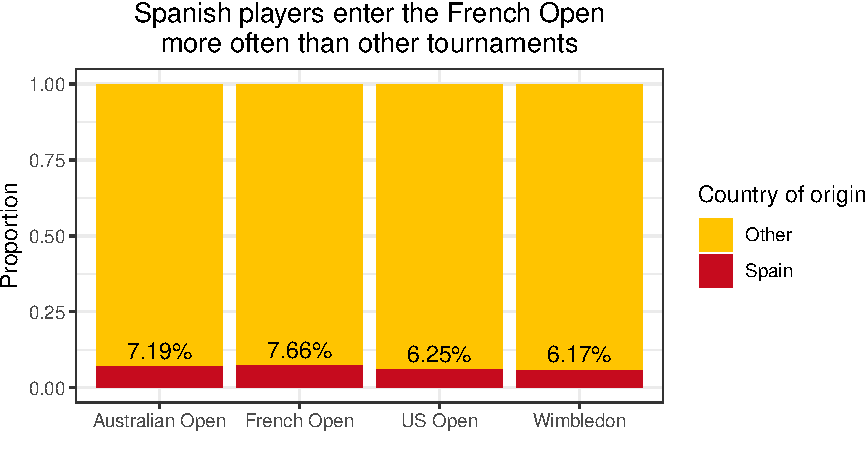
\includegraphics{paper-tennis_files/figure-latex/unnamed-chunk-3-1} \end{center}

\hypertarget{tall-players-and-aces}{%
\subsection{Tall players and aces}\label{tall-players-and-aces}}

Why the actual EFF won't fig.width work?

\begin{center}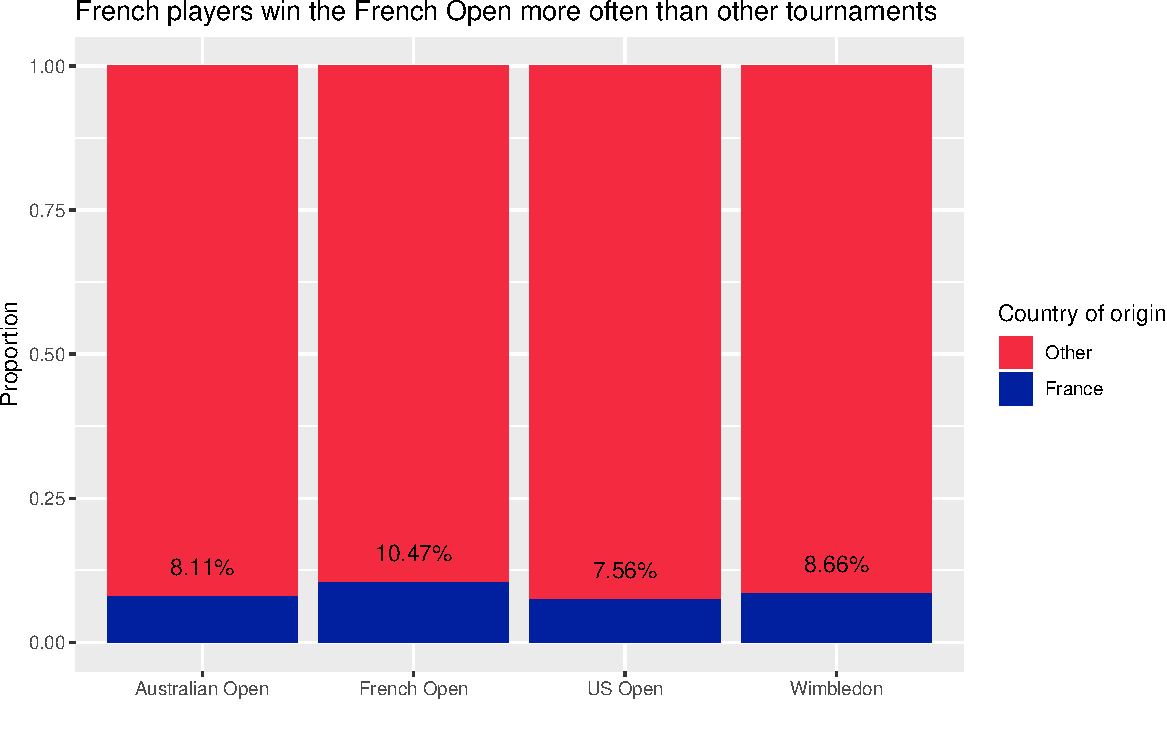
\includegraphics{paper-tennis_files/figure-latex/unnamed-chunk-4-1} \end{center}

\hypertarget{sec:methods}{%
\section{Methods}\label{sec:methods}}

\hypertarget{examining-individual-players}{%
\subsection{Examining individual
players}\label{examining-individual-players}}

\rowcolors{2}{gray!6}{white}
\begin{table}

\caption{\label{tab:table}\label{tab:three-gs-counts}Number of matches played for Nadal, Federer, and Williams from 2013-2017 at each of the grand slams.}
\centering
\begin{tabular}[t]{lrrr}
\hiderowcolors
\toprule
Tournament & Nadal & Federer & Williams\\
\midrule
\showrowcolors
Australian Open & 20 & 28 & 30\\
French Open & 29 & 14 & 23\\
US Open & 21 & 22 & 26\\
Wimbledon & 11 & 29 & 21\\
\rowcolor{lightgray}  \textbf{Total} & \textbf{81} & \textbf{93} & \textbf{100}\\
\bottomrule
\end{tabular}
\end{table}
\rowcolors{2}{white}{white}

In Table \ref{tab:three-gs-counts}, we display the number of matches
Nadal, Federer, and Williams have played from 2013-2017. Over that time
span, Nadal won 6 grand slams, Federer won 1, Williams won 8. Despite
this, Federer played more total matches in Nadal. All three players were
absent for exactly three slams during this time period due to external
factors (Nadal: (1 AO, 0 FO, 1 Wim, 1 USO), Federer: (0 AO, 2 FO, 0 Wim,
1 USO), Serena: (0 AO, 1 FO, 1 Wim, 1 USO)). Not unexpectedly, Nadal has
the most wins on clay (29), Federer has the most wins at Wimbledon (29)
and Williams the most on hardcourt (30 at AO and 21 at USO). Despite
having played more matches than Nadal, Federer only has 1 grand slam to
show compared to Nadal's six, which indicates that Federer made it
deeper into tournaments on average but had difficulties winning the
championships. For the WTA, Williams had her second most successful
five-year span at the grand slams over this time period, winning 8.

We fit individual linear models for these three individuals (subsetting
the data to their matches only), estimating the percent of points won in
a match using stepwise regression. The lower model is the percent of
points regressed on the opponent rank and indicator variables for court
type with the FO as the reference variable. The upper model is the lower
model with the additional variables of winner to unforced error ratio
(W/UE), average serve speed, percent aces, percent break points, percent
net points won, and their interaction effects with court type. We do not
display the full best fit models here, but they are available online. We
do report the effects (\(\pm 2 \cdot\) Std. Err.) of significant
variables and their interaction terms, adjusting for the other
covariates. Since we postulated that Nadal is best on clay, Federer on
grass, and Williams on hard court, specificically, AO, we use the FO,
Wim., and AO, respectively, as the reference variable in the model. For
Nadal and Federer we use forward-backwards stepwise regression, using
AIC as the criterion, beginning with the full model. For Williams, we
also use forwards-backwards stepwise regression but begin at the low
model since she has more missing data.

\hypertarget{nadal-king-of-clay-confirmed}{%
\subsection{Nadal: King of Clay:
confirmed}\label{nadal-king-of-clay-confirmed}}

Looking at Nadal individually, the model with the lowest AIC has
positive coefficients opponent rank, percent of aces, and percent of
break points won. It has negative coefficients for AO, USO, and Wim.
compared to FO and for percent of net points won. There are no
interaction effects in this model.

The standardized residuals plot shown in Figure \ref{fig:individ-resids}
(along with the other linear regression diagnostics plots not shown
here) shows that the model is a good fit for predicting the percent of
points won. For the significant variables (\(\alpha\) = 95\%), while
adjusting for the other variables, we expect percent of points won to be
\(0.034 \pm 0.028\) less at the AO and \(0.046 \pm 0.033\) less at Wim
compared to the FO; to increase by
\(1.5\times 10^{-4}\pm 1.3\times 10^{-4}\) for a one unit increase in
opponent rank; a \(0.0012\pm 5.6\times 10^{-4}\) increase for a .01
increase in percent of break points won; and to decrease by
\(8.8\times 10^{-4} \pm 5.5\times 10^{-4}\) for a .01 increase in
percent of net points won. As such, we see clear evidence Nadal performs
better at the FO compared to the other grand slams.

\hypertarget{federer-wimbledon-extraordinaire-debunked}{%
\subsection{Federer: Wimbledon extraordinaire:
debunked}\label{federer-wimbledon-extraordinaire-debunked}}

For Federer, the model with the lowest AIC has negative coefficients AO,
FO, and USO. vs Wim., and W/UE, It has positive coefficients for
opponent rank, percent of break points won, and all the interaction
terms: court and W/UE.

The standardized residuals plot shown in Figure \ref{fig:individ-resids}
shows that the model is a fairly good fit for predicting the percent of
points won, but almost seem to see two clusters of residuals splitting
with predicted point percentage of about 0.63. For the significant
variables (\(\alpha\) = 95\%), while adjusting for the other variables,
we expect percent of points won to be \(0.04 \pm 0.034\) less at AO
compared to the Wim.; \(0.058\pm 0.046\) less at FO compared to the
Wim.; \(0.007\pm 0.093\) less at USO compared to the Wim.; to decrease
by \(0.022 \pm 0.019\) for a one unit increase in W/UE at AO,
\(0.073 \pm 0.066\) for a one unit increase in W/UE at FO, and
\(0.041 \pm 0.033\) for a one unit increase in W/UE at USO. This is
strong evidence that Federer performs best at Wimbledon but possibly
does better at the USO, depending on his W/UE ratio.

\hypertarget{williams-hard-court-magician-only-debunked}{%
\subsection{Williams: hard court magician only:
debunked}\label{williams-hard-court-magician-only-debunked}}

\begin{figure}
\centering
\includegraphics{paper-tennis_files/figure-latex/resid plots-1.pdf}
\caption{\label{fig:individ-resids}Standardized residuals vs percent of
points won best fit model from forward-backwards stepwise regression for
Nadal's, Federer's, and William's, respectively.\}}
\end{figure}

For Williams, the model with the lowest AIC is the largest model of the
three selected 22 coefficients. Since Williams only has 59 observations,
we believe this model is overfitting and so caution against inference
with this model. It should also be noted that no women's point by point
data was recorded for 2015 so that year is excluded from this model. The
coefficients are court, opponent rank, W/UE, average serve speed,
percent aces, percent break points won, percent net points won, and
interaction effects with court and W/UE, court and average service
speed, court and percent aces, and court and break points won.

The standardized residuals plot shown in Figure \ref{fig:individ-resids}
shows that the model is a fair fit for predicting the percent of points
won, but we tend to overestimate the percent of points won in comparison
with Nadal. For the significant variables (\(\alpha\) = 95\(\%\)), while
adjusting for the other variables, we expect percent of points won to
increase by \(4.8\times 10^{-4} \pm 3.2\times 10^{-4}\) for a 1 unit
increase in oponent rank; to increase by \(0.034 \pm 0.02\) for a one
unit increase in W/UE at FO, to increase by \(0.092 \pm 0.045\) for a
one unit increase in W/UE at USO, and to increase by \(0.0038\pm 0.066\)
for a one unit increase in W/UE at Wim. compared to AO; to increase by
\(2\times 10^{-4}\pm 1.6\times 10^{-4}\) for a .01 increase in percent
of aces at the French Open; and to increase by \(0.0024 \pm 0.0011\) for
a .01 increase in percent of break points won at the French Open.

For this, we do not see that Williams is dominant on the hard courts
compared to the other courts. Rather, she has good results on all the
courts. Her significant interaction effects show that if she focuses on
acing her opponent and capitalizing on breakpoints, then she has a
better chance at winning more points than at the Australian Open.

\hypertarget{sec:discussion}{%
\section{Discussion}\label{sec:discussion}}

\hypertarget{sec:refs}{%
\section{References}\label{sec:refs}}

\footnotesize

\hypertarget{refs}{}
\leavevmode\hypertarget{ref-andersson2008}{}%
Andersson, Helena, Björn Ekblom, and Peter Krustrup. 2008. ``Elite
Football on Artificial Turf Versus Natural Grass: Movement Patterns,
Technical Standards, and Player Impressions'' 26 (February): 113--22.

\leavevmode\hypertarget{ref-egidi2018}{}%
Egidi, Leonardo, and Jonah Gabry. 2018. ``Bayesian Hierarchical Models
for Predicting Individual Performance in Soccer.'' \emph{Journal of
Quantitative Analysis in Sports} 14 (3). De Gruyter: 143--57.

\leavevmode\hypertarget{ref-gains2010}{}%
Gains, Graydon L, Andy N Swedenhjelm, Jerry L Mayhew, H Michael Bird,
and Jeremy J Houser. 2010. ``Comparison of Speed and Agility Performance
of College Football Players on Field Turf and Natural Grass.'' \emph{The
Journal of Strength \& Conditioning Research} 24 (10). LWW: 2613--7.

\leavevmode\hypertarget{ref-bbc2018}{}%
Jurejko, Jonathan. 2018. ``French Open 2018: Why does 'King of Clay'
Rafael Nadal reign supreme?'' Edited by BBC Sport at Roland Garros.
\url{https://www.bbc.com/sport/tennis/44385223}.

\leavevmode\hypertarget{ref-klaassen2003}{}%
Klaassen, Franc J.G.M., and Jan R. Magnus. 2003. ``Forecasting the
Winner of a Tennis Match.'' \emph{European Journal of Operational
Research} 148 (2): 257--67.
\url{https://doi.org/https://doi.org/10.1016/S0377-2217(02)00682-3}.

\leavevmode\hypertarget{ref-klaassen2001}{}%
Klaassen, Franc J.G.M., and Jan R Magnus. 2001. ``Are Points in Tennis
Independent and Identically Distributed? Evidence from a Dynamic Binary
Panel Data Model.'' \emph{Journal of the American Statistical
Association} 96 (454). Taylor \& Francis: 500--509.
\url{https://doi.org/10.1198/016214501753168217}.

\leavevmode\hypertarget{ref-knottenbelt2012}{}%
Knottenbelt, William J., Demetris Spanias, and Agnieszka M. Madurska.
2012. ``A Common-Opponent Stochastic Model for Predicting the Outcome of
Professional Tennis Matches.'' \emph{Computers \& Mathematics with
Applications} 64 (12): 3820--7.
\url{https://doi.org/https://doi.org/10.1016/j.camwa.2012.03.005}.

\leavevmode\hypertarget{ref-deuce2017}{}%
Kovalchik, Stephanie. 2017. \emph{Deuce: Resources for Analysis of
Professional Tennis Data}.

\leavevmode\hypertarget{ref-kovalchik2016}{}%
Kovalchik, Stephanie Ann. 2016. ``Searching for the Goat of Tennis Win
Prediction.'' \emph{Journal of Quantitative Analysis in Sports} 12 (3).
De Gruyter: 127--38.

\leavevmode\hypertarget{ref-leitner2009}{}%
Leitner, Christoph, Achim Zeileis, and Kurt Hornik. 2009. ``Is Federer
Stronger in a Tournamentwithout Nadal? An Evaluation of Odds and
Seedings for Wimbledon 2009.'' \emph{Austrian Journal of Statistics} 38
(4): 277--86.

\leavevmode\hypertarget{ref-mchale2011}{}%
McHale, Ian, and Alex Morton. 2011. ``A Bradley-Terry Type Model for
Forecasting Tennis Match Results.'' \emph{International Journal of
Forecasting} 27 (2): 619--30.
\url{https://doi.org/https://doi.org/10.1016/j.ijforecast.2010.04.004}.

\leavevmode\hypertarget{ref-five2015}{}%
Morris, Benjamin. 2015. ``Serena Williams and the Difference Between
All-Time Great and Greatest of All Time.'' Edited by FiveThirtyEight.
\url{https://fivethirtyeight.com/features/serena-williams-and-the-difference-between-all-time-great-and-greatest-of-all-time/}.

\leavevmode\hypertarget{ref-newton2005}{}%
Newton, Paul K, and Joseph B Keller. 2005. ``Probability of Winning at
Tennis I. Theory and Data.'' \emph{Studies in Applied Mathematics} 114
(3). Wiley Online Library: 241--69.

\leavevmode\hypertarget{ref-page2013}{}%
Page, Garritt L, Bradley J Barney, and Aaron T McGuire. 2013. ``Effect
of Position, Usage Rate, and Per Game Minutes Played on Nba Player
Production Curves.'' \emph{Journal of Quantitative Analysis in Sports} 9
(4). De Gruyter: 337--45.

\leavevmode\hypertarget{ref-theage2007}{}%
Paxinos, Stathi. 2007. ``Australian Open court surface is speeding up.''
Edited by The Age.
\url{https://www.theage.com.au/sport/tennis/australian-open-court-surface-is-speeding-up-20071120-ge6chj.html}.

\leavevmode\hypertarget{ref-sackmann2018}{}%
Sackmann, Jeff. 2018. ``Tennis Data Repositories.''
\url{https://github.com/JeffSackmann}.

\leavevmode\hypertarget{ref-thomas2013}{}%
Thomas, A. C., Samuel L. Ventura, Shane T. Jensen, and Stephen Ma. 2013.
``COMPETING Process Hazard Function Models for Player Ratings in Ice
Hockey.'' \emph{The Annals of Applied Statistics} 7 (3). Institute of
Mathematical Statistics: 1497--1524.
\url{http://www.jstor.org/stable/23566482}.


\end{document}
